\documentclass[journal,12pt,twocolumn]{IEEEtran}
\usepackage{setspace}
\usepackage{gensymb}
\usepackage{xcolor}
\usepackage{caption}
\singlespacing
\usepackage{siunitx}
\usepackage[cmex10]{amsmath}
\usepackage{mathtools}
\usepackage{hyperref}
\usepackage{amsthm}
\usepackage{mathrsfs}
\usepackage{txfonts}
\usepackage{stfloats}
\usepackage{cite}
\usepackage{cases}
\usepackage{subfig}
\usepackage{longtable}
\usepackage{multirow}
\usepackage{enumitem}
\usepackage{bm}
\usepackage{mathtools}
\usepackage{listings}
\usepackage{tikz}
\usetikzlibrary{shapes,arrows,positioning}
\usepackage{circuitikz}
\renewcommand{\vec}[1]{\boldsymbol{\mathbf{#1}}}
\DeclareMathOperator*{\Res}{Res}
\renewcommand\thesection{\arabic{section}}
\renewcommand\thesubsection{\thesection.\arabic{subsection}}
\renewcommand\thesubsubsection{\thesubsection.\arabic{subsubsection}}

\renewcommand\thesectiondis{\arabic{section}}
\renewcommand\thesubsectiondis{\thesectiondis.\arabic{subsection}}
\renewcommand\thesubsubsectiondis{\thesubsectiondis.\arabic{subsubsection}}
\hyphenation{op-tical net-works semi-conduc-tor}

\lstset{
language=Python,
frame=single, 
breaklines=true,
columns=fullflexible
}
\begin{document}
\theoremstyle{definition}
\newtheorem{theorem}{Theorem}[section]
\newtheorem{problem}{Problem}
\newtheorem{proposition}{Proposition}[section]
\newtheorem{lemma}{Lemma}[section]
\newtheorem{corollary}[theorem]{Corollary}
\newtheorem{example}{Example}[section]
\newtheorem{definition}{Definition}[section]
\newcommand{\BEQA}{\begin{eqnarray}}
\newcommand{\EEQA}{\end{eqnarray}}
\newcommand{\define}{\stackrel{\triangle}{=}}
\newcommand{\myvec}[1]{\ensuremath{\begin{pmatrix}#1\end{pmatrix}}}
\newcommand{\mydet}[1]{\ensuremath{\begin{vmatrix}#1\end{vmatrix}}}
\bibliographystyle{IEEEtran}
\providecommand{\nCr}[2]{\,^{#1}C_{#2}} % nCr
\providecommand{\nPr}[2]{\,^{#1}P_{#2}} % nPr
\providecommand{\mbf}{\mathbf}
\providecommand{\pr}[1]{\ensuremath{\Pr\left(#1\right)}}
\providecommand{\qfunc}[1]{\ensuremath{Q\left(#1\right)}}
\providecommand{\sbrak}[1]{\ensuremath{{}\left[#1\right]}}
\providecommand{\lsbrak}[1]{\ensuremath{{}\left[#1\right.}}
\providecommand{\rsbrak}[1]{\ensuremath{{}\left.#1\right]}}
\providecommand{\brak}[1]{\ensuremath{\left(#1\right)}}
\providecommand{\lbrak}[1]{\ensuremath{\left(#1\right.}}
\providecommand{\rbrak}[1]{\ensuremath{\left.#1\right)}}
\providecommand{\cbrak}[1]{\ensuremath{\left\{#1\right\}}}
\providecommand{\lcbrak}[1]{\ensuremath{\left\{#1\right.}}
\providecommand{\rcbrak}[1]{\ensuremath{\left.#1\right\}}}
\theoremstyle{remark}
\newtheorem{rem}{Remark}
\newcommand{\sgn}{\mathop{\mathrm{sgn}}}
\newcommand{\rect}{\mathop{\mathrm{rect}}}
\newcommand{\sinc}{\mathop{\mathrm{sinc}}}
\providecommand{\abs}[1]{\left\vert#1\right\vert}
\providecommand{\res}[1]{\Res\displaylimits_{#1}} 
\providecommand{\norm}[1]{\left\Vert#1\right\Vert}
\providecommand{\mtx}[1]{\mathbf{#1}}
\providecommand{\mean}[1]{E\left[ #1 \right]}
\providecommand{\fourier}{\overset{\mathcal{F}}{ \rightleftharpoons}}
\providecommand{\ztrans}{\overset{\mathcal{Z}}{ \rightleftharpoons}}
\providecommand{\system}[1]{\overset{\mathcal{#1}}{ \longleftrightarrow}}
\newcommand{\solution}{\noindent \textbf{Solution: }}
\providecommand{\dec}[2]{\ensuremath{\overset{#1}{\underset{#2}{\gtrless}}}}
\let\StandardTheFigure\thefigure
\def\putbox#1#2#3{\makebox[0in][l]{\makebox[#1][l]{}\raisebox{\baselineskip}[0in][0in]{\raisebox{#2}[0in][0in]{#3}}}}
     \def\rightbox#1{\makebox[0in][r]{#1}}
     \def\centbox#1{\makebox[0in]{#1}}
     \def\topbox#1{\raisebox{-\baselineskip}[0in][0in]{#1}}
     \def\midbox#1{\raisebox{-0.5\baselineskip}[0in][0in]{#1}}

\vspace{3cm}
\title{Circle Assignment}
\author{Gautam Singh}
\maketitle
\bigskip

\begin{abstract}
    This document contains the solution to Question 12 of 
    Exercise 5 in Chapter 10 of the class 9 NCERT textbook.
\end{abstract}

\begin{enumerate}
    \item Prove that a cyclic paralellogram is a rectangle.

    \solution Consider the points $\vec{P_i},\ 1 \le i \le 4$ on the 
    unit circle, where
    \begin{align}
        \vec{P_i} \triangleq \myvec{\cos{\theta_i}\\\sin{\theta_i}}
        \label{eq:P-def}
    \end{align}
    Now, since $P_1P_2P_3P_4$ form a parallelogram,
    \begin{align}
        \norm{\vec{P_1}-\vec{P_2}} &= \norm{\vec{P_3}-\vec{P_4}} \\
        \implies \vec{P_1}^\top\vec{P_2} &= \vec{P_3}^\top\vec{P_4}
        \label{eq:dot-prod-1}
    \end{align}
    and
    \begin{align}
        \norm{\vec{P_1}-\vec{P_4}} &= \norm{\vec{P_2}-\vec{P_3}} \\
        \implies \vec{P_1}^\top\vec{P_4} &= \vec{P_2}^\top\vec{P_3}
        \label{eq:dot-prod-2}
    \end{align}
    Also, it is given that the parallelogram is cyclic. So,
    \begin{align}
        \brak{\vec{P_4}-\vec{P_1}}^\top\brak{\vec{P_1}-\vec{P_2}} + \brak{\vec{P_4}-\vec{P_3}}^\top\brak{\vec{P_3}-\vec{P_2}} = 0
        \label{eq:cyclic}
    \end{align}
    Using \eqref{eq:dot-prod-1} and \eqref{eq:dot-prod-2} in \eqref{eq:cyclic}, 
    and noting that $\vec{P_i}^\top\vec{P_i} = 1,\ 1 \le i \le 4$,
    \begin{align}
        \vec{P_4}^\top\vec{P_1}-\vec{P_4}^\top\vec{P_2}+\vec{P_1}^\top\vec{P_2}-1 &= 0 \\
        \vec{P_4}^\top\vec{P_1}-\vec{P_4}^\top\vec{P_2}+\vec{P_1}^\top\vec{P_2}-\vec{P_1}^\top\vec{P_1} &= 0 \\
        \brak{\vec{P_4}-\vec{P_1}}^\top\brak{\vec{P_1}-\vec{P_2}} &= 0
        \label{eq:ortho}
    \end{align}
    Hence $P_1P_2 \perp P_1P_4$, and thus, the parallelogram is indeed a rectangle.
    The situation is demonstrated in Fig. \ref{fig:circle}, plotted by the Python
    code \texttt{codes/circle.py}.
    \begin{figure}[!ht]
        \centering
        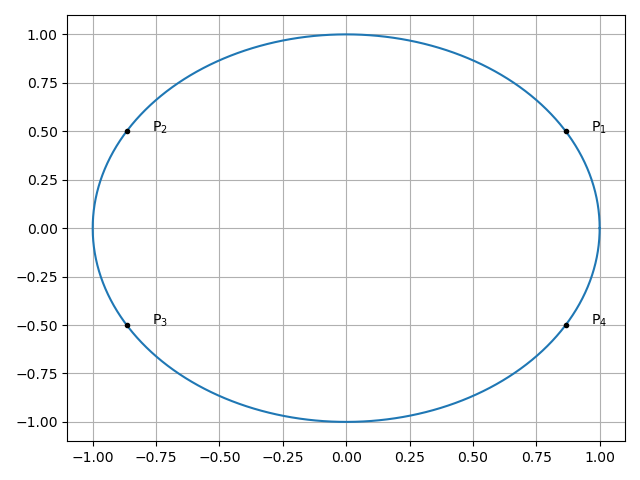
\includegraphics[width=\columnwidth]{figs/circle.png}
        \caption{$P_1P_2P_3P_4$ is a rectangle.}
        \label{fig:circle}
    \end{figure}
\end{enumerate}
\end{document}
